\documentclass[a4paper,12pt]{foi}

\renewcommand{\brojAutora}{1} % Broj autora rada (max. 6)

\renewcommand{\naslov}{Aplikacija za vođenje statistike skladišta i planiranje zaliha (strategije upravljanja zalihama - minimalne/maksimalne količine)} % Naslov rada

\renewcommand{\mentor}{Doc. dr. sc. Markus Schatten} % Ime i prezime mentora
\renewcommand{\kolegij}{Teorija baza podataka} % Naziv kolegija

\renewcommand{\autorA}{Marko Domladovac} % Ime i prezime prvog autora
\renewcommand{\brIndeksaA}{44532} % Broj indeksa prvog autora
% Odkomentirati ostale autore po potrebi
%\renewcommand{\autorB}{Ime Prezime}
%\renewcommand{\brIndeksaB}{33202}
%\renewcommand{\autorC}{Ime Prezime}
%\renewcommand{\brIndeksaC}{33203}
%\renewcommand{\autorD}{Ime Prezime}
%\renewcommand{\brIndeksaD}{33204}
%\renewcommand{\autorE}{Ime Prezime}
%\renewcommand{\brIndeksaE}{33205}
%\renewcommand{\autorF}{Ime Prezime}
%\renewcommand{\brIndeksaF}{33206}

\renewcommand{\vrstaRada}{Projekt} % Vrsta rada: Seminarski rad, Pristupni rad, Projekt ...



\begin{document}

\maketitle

\tableofcontents

\thispagestyle{empty}

\setcounter{page}{0}

\onehalfspacing

\chapter{Uvod}

Cilj i svrha projekta je izrada aplikacije za vođenje statistike skladišta i planiranja zaliha korištenjem strategije upravljanja zalihama (npr. minimalne/maksimalne količine, vremena između nabavki, ...).
Za bazu podataka će se koristiti PostgreSQL a za prezentacijski sloj .Net Core. Kako je .Net Core relativno novo htio sam isprobati kako .Net funkcionira u svijetu otvorenog koda. Dakle, ova aplikacija se treba moći vrtiti na svim operacijskim sustavima. Ja sam isprobao na Windowsima 10, Ubuntu 16.04 i  Mac OS X 10.7 Lion operacijskim sustavima i na svima radi.

\chapter{Opis aplikacijske domene}

Aplikacijska domena koju će se riješavati je upravljanje zalihama lijekova u bolnici. U bolnici je bitno da lijekovi uvijek  budu dostupni i zato je bitno upravljati zalihama istih. Osim samih količina, ovdje je bitan i faktor roka trajanja i mora se uzeti u obzir. Morati će se koristiti statistika korištenja kako bi se ispravno implementirale minimalne i maksimalne količine, kako s jedne strane nikada ne bi falilo i s druge strane kako se ne bi bacali lijekovi radi isteka roka trajanja jer je to gubitak resursa.
 
\paragraph{}
\underline{Korišteni koncepti su}:

\begin{itemize}
	\item Zaposlenik - osoba koja radi u bolnici u nabavi 
	\item Dokument - može biti primka ili narudžbenica, prema početnoj definiciji. Dokument može biti u sljedećim stanjima:
		\begin{enumerate}
			\item Zaprimljen
			\item U obradi
			\item Završen
			\item Otkazan
		\end{enumerate}
	\item Proizvod - u našem slučaju popis lijekova
	\item Stanje proizvoda - ovdje se implementira strategija minimalne/maksimalne količine. Odvojeno je od samog proizvoda kako bi popis proizvoda bio dostupan prilikom dohvata za preglede (potreban nam je samo naziv i id) i kako bi se optimirala sama aplikacija. Tu se nalaze polja minimalna i maksimalna količina, trenutno stanje, jedinica mjere i veza na proizvod, odnosno lijek.
\end{itemize}

\section{Proizvod}

Koncept "Proizvod" daje osnovne informacije o proizvodu i to putem sljedećih atributa: Naziv, Opis, Vrijednost, RokTrajanja.
U konceptu "Proizvod" navedene su sve specičnosti svakog pojedinog lijeka koji može doći u doticaj sa skladištem lijeka - bilo nabavom robe od dobavljača ili otpremom sa skladišta prilikom davanja lijeka pacijentu.

\section{Zaposlenik}

Koncept "Zaposlenik" obuhvaća sve zaposlene u bolnici. Zaposlenici bolnice  koji imaju doticaj s zaprimanjem i izdavanjem lijekova su najbitniji za aplikacijsku domenu koja se obrađuje jer će isti koristiti samu aplikaciju. Liječnik kada izdaje lijek onda se stanje smanjuje. Druga strana je zaprimanje lijekova prilikom dostizanja minimalne količine gdje se naručuju dostatne količine (razlika do maksimalne). Koncept je prikazan relacijom "Zaposlenik" sa sljedećim atributima: ID, Ime, Prezime, DatumRodjenja i KontaktID koje je poveznica na tablicu s kontaktima i ovdje se radi o vezi 1:1 ali nije dodano unutar same tablice jer se za poslovne partnere korisiti veze 1:N sa kontaktima pa je odabrana takva arhitektura sa posebnom tablicom s kontaktima.

\section{Dokument}

Jedan od najvažnijih, ako ne i najvažniji koncept je "Dokument". To je iz razloga jer će svaki ispravan dokument (ispravan dokument je onaj koji nije u stanju "otkazan") promijeniti stanje količine. Ukoliko se radi o vrsti dokumenta "Izdatnica" onda se količine smanjuju, a u slučaju primke te se količine povećavaju. Koncept dokumenta realiziran je pomoću tablice "Stavka\textunderscore Dokumenta" gdje imamo poveznicu na dokument i proizvod te količinu tog proizvoda vezano uz taj dokument. Koncept je iskazan relacijom "Dokument" sa sljedećim atributima:  ID, DatumKreiranje, DatumAzuriranja, ZaposlenikID, StatusID, VrstaID, Godina, a relacija "Stavka\textunderscore Dokumenta" ima sljedeće atribute: DokumentID, ProizvodID, Kolicina.

\section{Partner}

Jedan od četiri glavna kocepta je koncept "Partner". Koncept partner obuhvaća domenu dobavljača i pacijenata. Prilikom liječničkog pregleda kada se ustanovi da je potreban lijek i koji je to lijek izdaje se isti za pacijenta (vrsta partnera), dok je druga krajnost prilikom nabave lijeka gdje se naručuje od dobavljača što je druga vrsta partnera. Koncept partner može imati više kontakata i sukladno tome postoji vezna tablica "Partner\textunderscore Kontakt" koja povezuje koncept "Partner" i njegove kontakte. Osim toga postoji i poveznica na relaciju "Vrsta\textunderscore Partnera" koja govori o kojoj se vrsti partnera radi (dobavljač ili pacijent). U relaciji "Partner" postoje sljedeći atributi: ID, Naziv, DatumKreiranja, VrstaID, a "Partner\textunderscore Kontakt" poveznicu između kontakta i partnera tj. atribute: PartnerID i KontaktID koji su zapravo strani ključevi na navedene koncepte.

\section{Stanje Proizvoda}

Stanje proizvoda je najvažniji koncept vezan uz samu strategiju minimalne/maksimalne količine. Navedeni koncept nam govori o kojem se proizvodu radi, koja se jedinica mjere koristi, minimalna količina, maksimalna količina te njegovo trenutno stanje. Koncept "Stanje\textunderscore Proizvoda" je opisan sa sljedećim atributima: ID; MaksimalnaKolicina, MinimalnaKolicina, Stanje, JedinicaMjereID, ProizvodID.


\chapter{Teorijski uvod}

U središtu rada je baza podataka. Postoje razne vrste, no za implementaciju predmetne aplikacijske domene će se koristiti Aktivna i Temporalna baza podataka.

\section{Aktivna baza podataka}

Aktivna baza podataka uključuje aktivna pravila koja su najčešće u obliku: "Događaj - Uvjet - Akcija", eng. ECA ili "Event - Condition - Action".
Prednosti ovakvih baza podataka su da obogaćuju tradicionalne baze podataka sa mehanizmima za procesiranje pravila, a temelje se na okidačima. Ono što također omogućuju aktivne baze podataka su: uvjeti integriteta, pogledi, statistička pračenja, sigurnost baze podataka, sustavi temeljeni na znanju, ekspertni sustavi, upravljanje tokovima rada i dr. \citep[][]{Schatten2008}
Okidači omogućuju izvršavanje radnji na akcije upisa, ažuriranja ili brisanja podataka
iz nekih tablica. Npr. nakon što se promijeni stanje lijeka okidač aktivira provjeru s minimalnom i maksimalnom količinom te, ovisno o potrebi, šalje obavijest na email odgovorne osobe.

\section{Temporalne baze podataka}

Baza podataka sadrži podatke o organizaciji i njenim aktivnostima. Ona je osnova za razne aplikacije
od interesa za danu organizaciju. Konvencionalne baze podataka oblikovane su tako da sadrže najnovije
podatke,   tj.   tekuće   podatke.   Ažuriranjem   baze   podataka   ‘stare’   vrijednosti   se   eliminiraju   iz   baze
podataka.   Prema   tome,   baza   podataka   je   model   tekućeg   stanja   aplikacijske   domene   (snapshot   of
reality). Temporalne baze podataka  omogućuju reprezentaciju povijesti objekata \citep{Malekovic2017}

\paragraph{}

Temporalni relacijski model sastoji se od:
\begin{itemize}
	\item Temporalnih relacija
	\item Temporalne relacijske algebre
	\item Temporalnih uvjeta integriteta
\end{itemize}

Npr. zaposlenik je ima u određenom razdoblju jednu plaću, a u drugom ima drugi iznos. U temporalnoj tablici bi bila oba zapisa, dok u aktivnoj gdje je važno samo tekuće stanje bi bio samo jedan, najzadnji, zapis.


\chapter{Model baze podataka}

Na slici 4.1 prikazan je ERA model baze podataka. Model je dobiven obrnutin inženjeringom pomoću DbSchema alata. Baza podataka se sastoji od 12 tablica: 

\begin{itemize}
	\item Proizvod
	\item Stanje\textunderscore Proizvoda
	\item Jedinica\textunderscore Mjere
	\item Dokument
	\item Status\textunderscore Dokumenta
	\item Vrsta\textunderscore Dokumenta
	\item Zaposlenik
	\item Partner
	\item Kontakt
	\item Partner\textunderscore Kontakt
	\item Vrsta\textunderscore Partnera
\end{itemize}

\paragraph{}
Jaki objekti su Proizvod, Kontakt, Zaposlenik i Partner te šifrarnici (Vrsta\textunderscore Partnera, Vrsta\textunderscore Dokumenta, Jedinica\textunderscore Mjere i Status\textunderscore Dokumenta) jer ne ovise o nikome. Ostalo su slabe tablice. Partner\textunderscore Kontakt je povezujuća tablica jer Partner može imati više kontakata i zato što zaposlenik isto može imati kontakt pa da se ne prlja tablica s PartnerID koji može biti null ako je kontakt od zaposlenika ili u budućnosti od nečeg drugog.

\begin{figure}[h]
\centering 
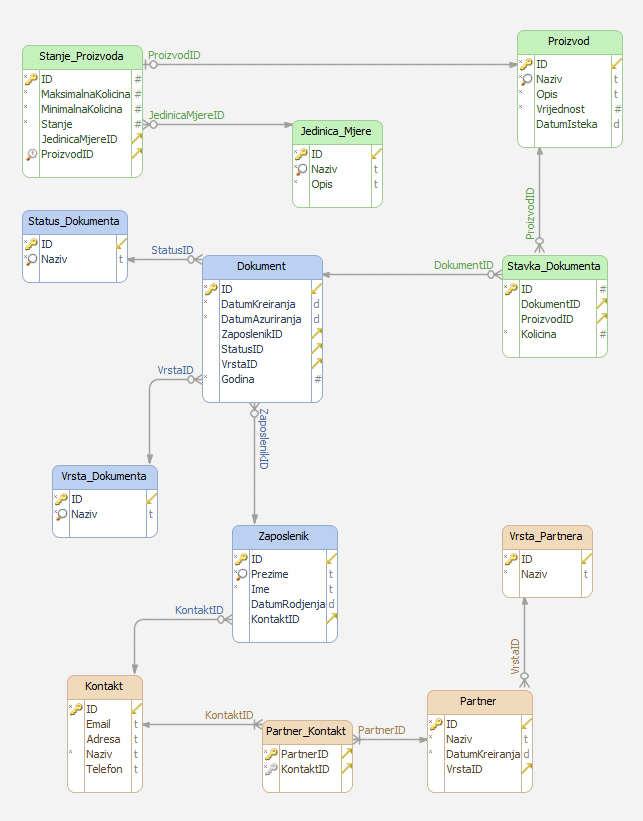
\includegraphics[width=0.95\textwidth]{model.png}
\caption{ERA model}
\label{slika-1}
\end{figure}

\section{Proizvod}

U tablicu se upisuju osnovne informacije o lijekovima koji su u upotrebi ili su bili u upotrebi ili budu u upotrebi. Osnovne informacije o proizvodu su: 

\begin{itemize}
	\item Naziv, 
	\item Opis,
	\item Vrijednost - vrijednost jedne jedinice mjere u HRK,
	\item RokTrajanja - važan kako bi se mogao raditi otpis (smanjuje stanje)
\end{itemize}

\section{Dokument}

Tablica Dokument nam služi za pohranu narudžbenice, primka i izdatnice. Ukoliko se dosegnu minimalne količine sustav će nas upozoriti da trebamo naručiti dostatne količine. Kreira se narudžbenica prema dobavljaču koja kada se provede stigne do bolnice i preuzima se gdje se onda stvara primka. Nakon zaprimanja ista roba postoji na stanju i može se dati pacijentu i to putem izdatnice. Tablica dokument sadrži informacije o datumu kreiranja, datumu ažuriranja, zaposleniku koji je zadnji radio na dokumentu, status dokumenta, vrsta dokumenta i godinu. Informacija godina je redundantan podataka ali nam služi za particioniranje podataka, no o tome nešto više u samom opisu implementacije.

\section{Zaposlenik}

Tablica Zaposlenik predstavlja zaposlenike bolnice. Bilo da se radi o referentima, liječnicima i sl. Tablica pruža osnovne informacije o zaposlenicima: 

\begin{itemize}
	\item Ime, 
	\item Prezime,
	\item DatumRodjenja - datum rođenja,
	\item KontakID - referencu na kontakt (1:1)
\end{itemize}

\section{Partner}

Tablica Partner obuhvaća sve dobavljače i pacijente koji dobivaju lijek i koji su neposredno povezani s promjenom stanja lijekova. Pacijenti djeluju direktno na smanjenje stanja lijekova, dok dobavljači na povećanje stanja lijekova. Tablica Partner sadržava sljedeće informacije: 

\begin{itemize}
	\item Naziv - naziv poduzeća ili Prezime, Ime ako je pacijent, 
	\item DatumKreiranja - datum kreiranja,
	\item VrstaID - vrsta partnera (dobavljač ili pacijent)
\end{itemize}

\section{Stanje Proizvoda}

Tablica Stanje\textunderscore Proizvoda je ključna za implementaciju strategije minimalne/maksimalne količine. Tablica sadrži sljedeće informacije: 

\begin{itemize}
	\item MaksimalnaKolicina - maksimalna dopuštena količina lijekova na stanju,
	\item MinimalnaKolicina -  minimalna dopuštena količina lijekova na stanju,
	\item Stanje - trenutno stanje na lageru,
	\item JedinicaMjereID - referenca na jedinicu mjere,
	\item ProizvodID - referenca na proizvod
\end{itemize}

\section{Stavka Dokumenta}

Tablica Stavka\textunderscore Dokumenta nam daje informacije o pojedinoj stavci određenog dokumenta, bilo da se radi o narudžbenici, primci, izdatnici i sl. Sadrži sljedeće informacije:

\begin{itemize}
	\item DokumentID - referencu na dokument kojem pripada,
	\item ProizvodID - referencu na proizvod o kojem se radi,
	\item Kolicina - količina proizvoda
\end{itemize}

\section{Kontakt}

Tablica kontakt sadrži kontakt informacije:

\begin{itemize}
	\item Email,
	\item Adresa,
	\item Naziv,
	\item Telefon
\end{itemize}

\section{Šifrarnici}

Tablice Status\textunderscore Dokumenta, Vrsta\textunderscore Partnera, Jedinica\textunderscore Mjere, Vrsta\textunderscore Dokumenta su šifrarnici i sadrže samo naziv i opis ukoliko je potrebno. 

\chapter{Implementacija}

\section{Kreiranje sheme baze podataka}

Prije svega potrebno je kreirati bazu podataka. Kreiranje baze podataka u PostgreSQL-u, točnije u SQL jeziku, se radi sa sljedećom naredbom:

\definecolor{lbcolor}{rgb}{0.9,0.9,0.9}
\lstset{commentstyle=\textit,language=SQL}
\lstset{backgroundcolor=\color{lbcolor},rulecolor=}
\begin{lstlisting}[frame=tb]{}
 CREATE DATABASE tbpfoi WITH TEMPLATE = tbp_template 
 	ENCODING = 'UTF8' 
 	LC_COLLATE = 'Croatian_Croatia.1250' 
 	LC_CTYPE = 'Croatian_Croatia.1250';
 ALTER DATABASE tbpfoi OWNER TO marko;
\end{lstlisting}

Nakon što je baza podataka kreirana i pridružena željenom korisniku, mogu se kreirati tablice:

\definecolor{lbcolor}{rgb}{0.9,0.9,0.9}
\lstset{commentstyle=\textit,language=SQL}
\lstset{backgroundcolor=\color{lbcolor},rulecolor=}
\begin{lstlisting}[frame=tb]{}
 CREATE TABLE "Dokument" (
    "ID" integer NOT NULL,
    "DatumKreiranja" timestamp without time zone 
    	DEFAULT now() NOT NULL,
    "DatumAzuriranja" timestamp without time zone 
    	DEFAULT now() NOT NULL,
    "ZaposlenikID" integer,
    "StatusID" integer,
    "VrstaID" integer,
    "Godina" smallint DEFAULT 2017 NOT NULL
 );
 
 CREATE TABLE "Jedinica_Mjere" (
    "ID" integer NOT NULL,
    "Naziv" character varying(20) NOT NULL,
    "Opis" character varying(128) NOT NULL
 );
 
 CREATE TABLE "Kontakt" (
    "ID" integer NOT NULL,
    "Email" character varying(64),
    "Adresa" character varying(128),
    "Naziv" character varying(32) NOT NULL,
    "Telefon" character varying(15)
 );
 
 CREATE TABLE "Partner" (
    "ID" integer NOT NULL,
    "Naziv" character varying(64) NOT NULL,
    "DatumKreiranja" time without time zone NOT NULL,
    "VrstaID" integer
 );
 
 CREATE TABLE "Partner_Kontakt" (
    "PartnerID" integer NOT NULL,
    "KontaktID" integer NOT NULL
 );
 
 CREATE TABLE "Proizvod" (
    "ID" integer NOT NULL,
    "Naziv" character varying(20) NOT NULL,
    "Opis" character varying(128) NOT NULL,
    "Vrijednost" real NOT NULL,
    "RokTrajanja" smallint NOT NULL
 );
 
 CREATE TABLE "Stanje_Proizvoda" (
    "ID" integer NOT NULL,
    "MaksimalnaKolicina" double precision NOT NULL,
    "MinimalnaKolicina" double precision NOT NULL,
    "Stanje" double precision DEFAULT 0 NOT NULL,
    "JedinicaMjereID" integer,
    "ProizvodID" integer,
    CONSTRAINT "StanjeProizvoda_MaksimalnaKolicina_check" 
    	CHECK (("MaksimalnaKolicina" > (0)::double precision)),
    CONSTRAINT "StanjeProizvoda_MinimalnaKolicina_check" 
    	CHECK (("MinimalnaKolicina" >= (0)::double precision)),
    CONSTRAINT "StanjeProizvoda_Stanje_check" 
    	CHECK (("Stanje" >= (0)::double precision)),
    CONSTRAINT "StanjeProizvoda_check" 
    	CHECK (("MaksimalnaKolicina" > "MinimalnaKolicina")),
    CONSTRAINT "StanjeProizvoda_check1" 
    	CHECK (("MaksimalnaKolicina" > "Stanje")),
    CONSTRAINT "StanjeProizvoda_check2" 
    	CHECK (("Stanje" >= "MinimalnaKolicina"))
 );
 
 CREATE TABLE "Stavka_Dokumenta" (
    "ID" integer NOT NULL,
    "DokumentID" integer,
    "ProizvodID" integer,
    "Kolicina" double precision NOT NULL,
    CONSTRAINT "StavkaDokumenta_Kolicina_check" 
    	CHECK (("Kolicina" > (0)::double precision))
 );
 
 CREATE TABLE "Vrsta_Dokumenta" (
    "ID" integer NOT NULL,
    "Naziv" character varying(20) NOT NULL
 );
 
 CREATE TABLE "Vrsta_Partnera" (
    "ID" integer NOT NULL,
    "Naziv" character varying(64) NOT NULL
 );
 
 CREATE TABLE "Zaposlenik" (
    "ID" integer NOT NULL,
    "Prezime" character varying(32) NOT NULL,
    "Ime" character varying(32) NOT NULL,
    "DatumRodjenja" date,
    "KontaktID" integer,
    CONSTRAINT "CK_Rodjenje" 
    	CHECK (("DatumRodjenja" < now()))
 );
 
 ALTER TABLE ONLY "Dokument"
    ADD CONSTRAINT "PK_Dokument" PRIMARY KEY ("ID");

 ALTER TABLE ONLY "Jedinica_Mjere"
    ADD CONSTRAINT "PK_JedinicaMjere" PRIMARY KEY ("ID");

 ALTER TABLE ONLY "Proizvod"
    ADD CONSTRAINT "PK_Proizvod" PRIMARY KEY ("ID");

 ALTER TABLE ONLY "Stanje_Proizvoda"
    ADD CONSTRAINT "PK_StanjeProizvoda" PRIMARY KEY ("ID");

 ALTER TABLE ONLY "Status_Dokumenta"
    ADD CONSTRAINT "PK_StatusDokumenta" PRIMARY KEY ("ID");

 ALTER TABLE ONLY "Stavka_Dokumenta"
    ADD CONSTRAINT "PK_StavkaDokumenta" PRIMARY KEY ("ID");

 ALTER TABLE ONLY "Vrsta_Dokumenta"
    ADD CONSTRAINT "PK_VrstaDokumenta" PRIMARY KEY ("ID");

 ALTER TABLE ONLY "Zaposlenik"
    ADD CONSTRAINT "PK_Zaposlenik" PRIMARY KEY ("ID");
	
 ALTER TABLE ONLY "Partner_Kontakt"
    ADD CONSTRAINT "Partner_Kontakt_pkey" 
    PRIMARY KEY ("PartnerID", "KontaktID");

 ALTER TABLE ONLY "Stanje_Proizvoda"
    ADD CONSTRAINT "StanjeProizvoda_ProizvodID_key" 
    UNIQUE ("ProizvodID");

 ALTER TABLE ONLY "Partner"
    ADD CONSTRAINT dobavljac_pkey PRIMARY KEY ("ID");
	
 ALTER TABLE ONLY "Kontakt"
    ADD CONSTRAINT kontakt_pkey PRIMARY KEY ("ID");

 ALTER TABLE ONLY "Vrsta_Partnera"
    ADD CONSTRAINT vrsta_dobavljaca_pkey PRIMARY KEY ("ID");

 CREATE INDEX "JedinicaMjere_Naziv" ON "Jedinica_Mjere" 
 	USING btree ("Naziv");

 CREATE INDEX "Proizvod_Naziv" ON "Proizvod" 
 	USING btree ("Naziv");

 CREATE INDEX "StatusDokumenta_Naziv" ON "Status_Dokumenta" 
 	USING btree ("Naziv");

 CREATE INDEX "VrstaDokumenta_Naziv" ON "Vrsta_Dokumenta" 
 	USING btree ("Naziv");

 CREATE INDEX "Zaposlenik_Prezime" ON "Zaposlenik" 
 	USING btree ("Prezime"); 	

 ALTER TABLE ONLY "Partner"
    ADD CONSTRAINT "Dobavljac_Vrsta" FOREIGN KEY ("VrstaID") 
    REFERENCES "Vrsta_Partnera"("ID");

 ALTER TABLE ONLY "Dokument"
    ADD CONSTRAINT "Dokument_StatusID_fkey" FOREIGN KEY ("StatusID") 
    REFERENCES "Status_Dokumenta"("ID");

 ALTER TABLE ONLY "Dokument"
    ADD CONSTRAINT "Dokument_VrstaID_fkey" FOREIGN KEY ("VrstaID") 
    REFERENCES "Vrsta_Dokumenta"("ID");

 ALTER TABLE ONLY "Dokument"
    ADD CONSTRAINT "Dokument_ZaposlenikID_fkey" 
    FOREIGN KEY ("ZaposlenikID") REFERENCES "Zaposlenik"("ID");

 ALTER TABLE ONLY "Partner_Kontakt"
    ADD CONSTRAINT "Kontakt" FOREIGN KEY ("KontaktID") 
    REFERENCES "Kontakt"("ID");

 ALTER TABLE ONLY "Partner_Kontakt"
    ADD CONSTRAINT "Partner" FOREIGN KEY ("PartnerID") 
    REFERENCES "Partner"("ID");

 ALTER TABLE ONLY "Stanje_Proizvoda"
    ADD CONSTRAINT "StanjeProizvoda_JedinicaMjereID_fkey" 
    FOREIGN KEY ("JedinicaMjereID") REFERENCES "Jedinica_Mjere"("ID");

 ALTER TABLE ONLY "Stanje_Proizvoda"
    ADD CONSTRAINT "StanjeProizvoda_ProizvodID_fkey" 
    FOREIGN KEY ("ProizvodID") REFERENCES "Proizvod"("ID");

 ALTER TABLE ONLY "Stavka_Dokumenta"
    ADD CONSTRAINT "StavkaDokumenta_DokumentID_fkey" 
    FOREIGN KEY ("DokumentID") REFERENCES "Dokument"("ID");

 ALTER TABLE ONLY "Stavka_Dokumenta"
    ADD CONSTRAINT "StavkaDokumenta_ProizvodID_fkey" 
    FOREIGN KEY ("ProizvodID") REFERENCES "Proizvod"("ID");

 ALTER TABLE ONLY "Zaposlenik"
    ADD CONSTRAINT "Zaposlenik_Kontakt" 
    FOREIGN KEY ("KontaktID") REFERENCES "Kontakt"("ID");
    
\end{lstlisting}

Ovisno o verziji PostgreSQL-a dodaje se i automatsko dodavanje brojeva primarnom ključu. Može se koristiti ključna riječ serial ili napraviti slijed. Ovdje je kreiran slijed i na primjeru koda će se pokazati kako se kreira:

\definecolor{lbcolor}{rgb}{0.9,0.9,0.9}
\lstset{commentstyle=\textit,language=SQL}
\lstset{backgroundcolor=\color{lbcolor},rulecolor=}
\begin{lstlisting}[frame=tb]{}
 CREATE SEQUENCE "naziv_slijeda"
    START WITH 1
    INCREMENT BY 1
    NO MINVALUE
    NO MAXVALUE
    CACHE 1;
    
 ALTER SEQUENCE "naziv_slijeda" OWNED BY "tablica"."ID";
 
\end{lstlisting}

Nakon kreiranja struktura same baze podataka dodaje se dinamika u obliku okidača i funkcija: 

\definecolor{lbcolor}{rgb}{0.9,0.9,0.9}
\lstset{commentstyle=\textit,language=SQL}
\lstset{backgroundcolor=\color{lbcolor},rulecolor=}
\begin{lstlisting}[frame=tb]{}
 CREATE SEQUENCE "naziv_slijeda"
    START WITH 1
    INCREMENT BY 1
    NO MINVALUE
    NO MAXVALUE
    CACHE 1;
    
 ALTER SEQUENCE "naziv_slijeda" OWNED BY "tablica"."ID";
 
\end{lstlisting}

Nakon definiranja tablica potrebno je definirati funkcije, okidače, pravila i ograničenja.

Okidač za izdvajanje godine služi za particioniranje po godini radi optimizacije. Da bi particioniranje bilo uspješno, prilikom upita se pojedine particije isključuju. Tako ćemo ovdje vrlo jednostavno izvršavati upit za dokumente po godinama. Ovo bi trebalo daleko kompleksnije izgraditi no trenutna implementacija služi samo kao primjer: 


\definecolor{lbcolor}{rgb}{0.9,0.9,0.9}
\lstset{commentstyle=\textit,language=SQL}
\lstset{backgroundcolor=\color{lbcolor},rulecolor=}
\begin{lstlisting}[frame=tb]{}
 CREATE FUNCTION public.izdvoji_godinu()
    RETURNS trigger
    LANGUAGE 'plpgsql'
    COST 100
    VOLATILE NOT LEAKPROOF 
    ROWS 0
 AS $BODY$
 
    DECLARE 
    BEGIN 
        NEW."Godina" := EXTRACT(YEAR FROM NEW."DatumAzuriranja");
        RETURN NEW;
    END; 
    
 $BODY$;

 CREATE TRIGGER umetni_godinu
    BEFORE INSERT OR UPDATE 
    ON public."Dokument"
    FOR EACH ROW
    EXECUTE PROCEDURE public.izdvoji_godinu();

\end{lstlisting} 

\begin{figure}[h]
\centering 
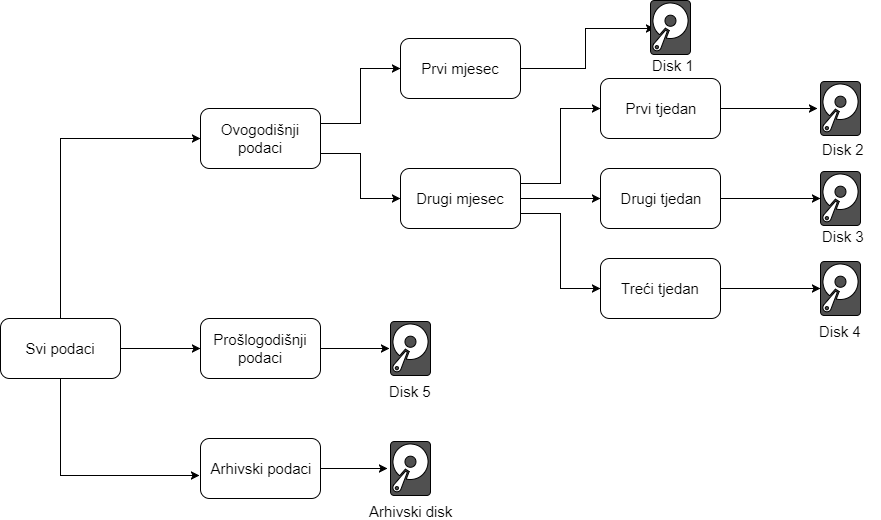
\includegraphics[width=0.95\textwidth]{particioniranje.png}
\caption{Raspodjela podataka po particijama i podparticijama}
\label{slika-2}
\end{figure}

Horizontalno particioniranje ili particioniranje po redcima jest
podjela podataka u kojoj se različiti redci nalaze u različitim tablicama
(koje nazivamo particijama tablice). Korištenjem unije
nad razdvojenim podacima dolazimo do ukupnog seta podataka.
Kod spajanja podataka unijom performanse će biti skoro identične
kao i kod čitanja iz jedne velike tablice ako se particioniranje radi
unutar istog servera. Česta je primjena horizontalnog particioniranja
razdvajanje podataka po serverima, što se u praksi zove distribuirano
particioniranje. Distribuirano particioniranje nije pogodno
za upite gdje je potrebno unirati sve podatke, ali zato drastično
ubrzava upite kod kojih se upit usmjerava na samo jednu particiju.

Primjer particije nad dokumentima: 


\definecolor{lbcolor}{rgb}{0.9,0.9,0.9}
\lstset{commentstyle=\textit,language=SQL}
\lstset{backgroundcolor=\color{lbcolor},rulecolor=}
\begin{lstlisting}[frame=tb]{}

 --Tablice particija
 CREATE TABLE Dokument_2016
 (
 	PRIMARY KEY("Godina", "ID"),
 	CHECK(godina=2016)
 ) INHERITS ("Dokument");

 CREATE TABLE Dokument_2017
 (
 	PRIMARY KEY("Godina", "ID"),
 	CHECK(godina=2017)
 ) INHERITS ("Dokument");

 --Pravila za unos:
 CREATE RULE unos_dokumenta_2016 AS
	ON INSERT TO "Dokument"
 	WHERE (godina = 2016)
 	DO INSTEAD INSERT INTO Dokument_2016 VALUES(NEW.*);
 
 CREATE RULE unos_dokumenta_2017 AS
 	ON INSERT TO "Dokument"
 	WHERE (godina = 2017)
 	DO INSTEAD INSERT INTO Dokument_2017 VALUES(NEW.*);


 --Nakon takvog kreiranja upiti se mogu optimizirati. npr.:
 SELECT * FROM "Dokument" WHERE "Godina" < 2017

 --Unosi isto zavrsavaju na pravom mjestu  
 INSERT INTO "Dokument" VALUES(1,1,1);
\end{lstlisting}

U nastavku će se opisati okidači koji su važni za implementaciju strategije minimalne/maksimalne količine. Isto je moguće implementirati i na aplikacijskoj razini, no ovdje zbog same svrhe kolegija je odabrana implementacija putem okidača. Nije uvijek dobro raditi stvari s okidačima, posebno ako se radi o kompleksnom sustavu jer znaju biti teški za održavati i debugirati. Prvi okidač takve vrste bude mijenjao stanje proizvoda prilikom dodavanja dokumenta. Ako je dokument primka onda se stanje povećava, a ako je dokument izdatnica onda se stanje smanjuje. Kod je prikazan ispod:

\definecolor{lbcolor}{rgb}{0.9,0.9,0.9}
\lstset{commentstyle=\textit,language=SQL}
\lstset{backgroundcolor=\color{lbcolor},rulecolor=}
\begin{lstlisting}[frame=tb]{}
 CREATE FUNCTION dodavanje_stavke_stanje() RETURNS TRIGGER AS $$
 DECLARE
 vd_id integer;
 vd_naziv varchar(30);
 kol integer;

 BEGIN

 SELECT "VrstaID" into vd_id FROM "Dokument" 
 	WHERE "ID" = NEW."DokumentID";
 	
 SELECT "Naziv" into vd_naziv FROM "Vrsta_Dokumenta" 
 	WHERE "ID" = vd_id;

 IF (vd_naziv = 'Primka') then kol = NEW."Kolicina";
 ELSIF (vd_naziv = 'Izdatnica') then kol = -1 * NEW."Kolicina";
 ELSE kol = 0;
 END IF;

 UPDATE "Stanje_Proizvoda" SET "Stanje" = "Stanje" + kol 
 	WHERE "ProizvodID" =    NEW."ProizvodID";

 RETURN NEW;
 END;
 $$ language plpgsql ;

 CREATE TRIGGER dokument_stanje
    AFTER INSERT OR UPDATE 
    ON public."Stavka_Dokumenta"
    FOR EACH ROW
    EXECUTE PROCEDURE public.primka_stanje();
\end{lstlisting}

Osim samog dodavanja jako je važno paziti na brisanje. Kako je normalno da se stavke mogu ukloniti, moramo se pobrinuti ili u aplikaciji ili u okidaču da je stanje točno. Kod je prikazan ispod:

\definecolor{lbcolor}{rgb}{0.9,0.9,0.9}
\lstset{commentstyle=\textit,language=SQL}
\lstset{backgroundcolor=\color{lbcolor},rulecolor=}
\begin{lstlisting}[frame=tb]{}
 CREATE OR REPLACE FUNCTION brisanje_stavki_stanje()
	RETURNS TRIGGER AS
 $$
 
 DECLARE
 vd_id integer;
 vd_naziv varchar(30);
 kol integer;

 BEGIN

 SELECT "VrstaID" into vd_id FROM "Dokument" WHERE "ID" = OLD."DokumentID";
 SELECT "Naziv" into vd_naziv FROM "Vrsta_Dokumenta" WHERE "ID" = vd_id;

 IF (vd_naziv = 'Izdatnica') then kol = OLD."Kolicina";
 ELSIF (vd_naziv = 'Primka') then kol = -1 * OLD."Kolicina";
 ELSE kol = 0;
 END IF;

 UPDATE "Stanje_Proizvoda" SET "Stanje" = "Stanje" + kol WHERE "ProizvodID" = OLD."ProizvodID";

 RETURN OLD;
 END;

 $$
 LANGUAGE plpgsql;

 CREATE TRIGGER brisanje_stavki
    AFTER DELETE
    ON public."Stavka_Dokumenta"
    FOR EACH ROW
    EXECUTE PROCEDURE public.brisanje_stavki_stanje();
    
\end{lstlisting}

Sljedeće je implementacija same aplikacije. Kako je odabrana tehnologija .Net Core onda je iskorišten Entity Framework kao ORM. Kako već postoji baza podataka, potrebno je izgenerirati klase i kontekst. Za to je potrebno nekoliko paketa od kojih su najvažnija dva za sam rad s PostgreSQL bazom:

\begin{itemize}
	\item Npgsql.EntityFrameworkCore.PostgreSQL
	\item Npgsql.EntityFrameworkCore.PostgreSQL.Design
\end{itemize}

Ostalo su paketi vezani uz samu aplikaciju, entity framework i sl. Sam model jedne tablice je prikazan kao POCO klasa sa proširenjima poput kolekcije ukoliko se radi o 1:N vezi ili drugoj klasi koja je šifrarnik, no najbolje je pogledati na primjeru klase Dokument koja implementira većinu mogućnosti:

\begin{lstlisting}[language={[Sharp]C}]
 using System;
 using System.Collections.Generic;

 namespace Web.Models
 {
    public partial class Dokument
    {
        public Dokument()
        {
            StavkaDokumenta = new HashSet<StavkaDokumenta>();
        }

        public int Id { get; set; }
        public DateTime DatumKreiranja { get; set; }
        public DateTime DatumAzuriranja { get; set; }
        public int? ZaposlenikId { get; set; }
        public int? StatusId { get; set; }
        public int? VrstaId { get; set; }
        public short Godina { get; set; }

        public virtual ICollection<StavkaDokumenta> 
        	StavkaDokumenta { get; set; }
        public virtual StatusDokumenta Status { get; set; }
        public virtual VrstaDokumenta Vrsta { get; set; }
        public virtual Zaposlenik Zaposlenik { get; set; }
    }
 }

\end{lstlisting}

Kao što je vidljivo klasa je parcijalna i to s razlogom. Kako je to generirana klasa direktno iz baze podataka, nakon svakog novog generiranja (npr. prilikom promjene strukture) bi se bilo kakav dodatak obrisao. Zašto bi se uopće radile izmjene? Izmjene su potrebne i to najčešće se koristi anotacija, npr. za automatsko imenovanje labela, jer ukoliko se to ne napravi u ptredolške se stavi pretpostavljeni naziv (u gornjem primjeru bi za vrstu u labeli pisalo VrstaID) što se često ne želi. Ispod na primjeru je prikazan drugi dio ove klase koji je odvojen da ne bi bio prebrisan, važno je samo da je u istom namespace-u:

\begin{lstlisting}[language={[Sharp]C}]
using Microsoft.AspNetCore.Mvc;
using System;
using System.ComponentModel;

namespace Web.Models
{
    [ModelMetadataType(typeof(DokumentMetaData))]
    public partial class Dokument
    {  }

    public class DokumentMetaData
    {

        [DisplayName("Datum kreiranja")]
        public DateTime DatumKreiranja { get; set; }

        [DisplayName("Datum azuriranja")]
        public DateTime DatumAzuriranja { get; set; }

        [DisplayName("Zaposlenik")]
        public int? ZaposlenikId { get; set; }

        [DisplayName("Status")]
        public int? StatusId { get; set; }

        [DisplayName("Vrsta")]
        public int? VrstaId { get; set; }
    }
}
\end{lstlisting}

I na isti način se implementiraju ostale tablice u obliku klasa. Najvažniji dio da bi se sve to povezalo je kontekst baze podataka. Unutar konteksta se opisuje komunikacija, specifičnosti i sl. Implementacija konteksta predmetne aplikacije je:

\begin{lstlisting}[language={[Sharp]C}]
using System;
using Microsoft.EntityFrameworkCore;
using Microsoft.EntityFrameworkCore.Metadata;

namespace Web.Models
{
    public partial class tbpfoiContext : DbContext
    {
        public virtual DbSet<Dokument> Dokument { get; set; }
        public virtual DbSet<JedinicaMjere> JedinicaMjere { get; set; }
        public virtual DbSet<Kontakt> Kontakt { get; set; }
        public virtual DbSet<Partner> Partner { get; set; }
        public virtual DbSet<PartnerKontakt> 
        	PartnerKontakt { get; set; }
        	
        public virtual DbSet<Proizvod> Proizvod { get; set; }
        public virtual DbSet<StanjeProizvoda> 
        	StanjeProizvoda { get; set; }
        	
        public virtual DbSet<StatusDokumenta> 
        	StatusDokumenta { get; set; }
        	
        public virtual DbSet<StavkaDokumenta> 
        	StavkaDokumenta { get; set; }
        	
        public virtual DbSet<VrstaDokumenta> 
        	VrstaDokumenta { get; set; }
        	
        public virtual DbSet<VrstaPartnera> VrstaPartnera { get; set; }
        public virtual DbSet<Zaposlenik> Zaposlenik { get; set; }

        public tbpfoiContext(DbContextOptions<tbpfoiContext> options)
   		: base(options) { }

        protected override void OnModelCreating
        	(ModelBuilder modelBuilder)
        {
            modelBuilder.Entity<Dokument>(entity =>
            {
                entity.Property(e => e.Id).HasColumnName("ID");

                entity.Property(e => e.DatumAzuriranja)
                	.HasDefaultValueSql("now()");

                entity.Property(e => e.DatumKreiranja)
                	.HasDefaultValueSql("now()");

                entity.Property(e => e.Godina)
                	.HasDefaultValueSql("2017");

                entity.Property(e => e.StatusId)
                	.HasColumnName("StatusID");

                entity.Property(e => e.VrstaId)
                	.HasColumnName("VrstaID");

                entity.Property(e => e.ZaposlenikId)
                	.HasColumnName("ZaposlenikID");

                entity.HasOne(d => d.Status)
                    .WithMany(p => p.Dokument)
                    .HasForeignKey(d => d.StatusId)
                    .HasConstraintName("Dokument_StatusID_fkey");

                entity.HasOne(d => d.Vrsta)
                    .WithMany(p => p.Dokument)
                    .HasForeignKey(d => d.VrstaId)
                    .HasConstraintName("Dokument_VrstaID_fkey");

                entity.HasOne(d => d.Zaposlenik)
                    .WithMany(p => p.Dokument)
                    .HasForeignKey(d => d.ZaposlenikId)
                    .HasConstraintName("Dokument_ZaposlenikID_fkey");
            });

            modelBuilder.Entity<JedinicaMjere>(entity =>
            {
                entity.ToTable("Jedinica_Mjere");

                entity.HasIndex(e => e.Naziv)
                    .HasName("JedinicaMjere_Naziv");

                entity.Property(e => e.Id)
                    .HasColumnName("ID")
                    .HasDefaultValueSql
                    ("nextval('\"JedinicaMjere_ID_seq\"'::regclass)");

                entity.Property(e => e.Naziv)
                    .IsRequired()
                    .HasColumnType("varchar")
                    .HasMaxLength(20);

                entity.Property(e => e.Opis)
                    .IsRequired()
                    .HasColumnType("varchar")
                    .HasMaxLength(128);
            });

            modelBuilder.Entity<Kontakt>(entity =>
            {
                entity.Property(e => e.Id)
                    .HasColumnName("ID")
                    .HasDefaultValueSql
                    ("nextval('\"kontakt_ID_seq\"'::regclass)");

                entity.Property(e => e.Adresa)
                    .HasColumnType("varchar")
                    .HasMaxLength(128);

                entity.Property(e => e.Email)
                    .HasColumnType("varchar")
                    .HasMaxLength(64);

                entity.Property(e => e.Naziv)
                    .IsRequired()
                    .HasColumnType("varchar")
                    .HasMaxLength(32);

                entity.Property(e => e.Telefon)
                    .HasColumnType("varchar")
                    .HasMaxLength(15);
            });

            modelBuilder.Entity<Partner>(entity =>
            {
                entity.Property(e => e.Id)
                    .HasColumnName("ID")
                    .HasDefaultValueSql
                    ("nextval('\"dobavljac_ID_seq\"'::regclass)");

                entity.Property(e => e.DatumKreiranja)
                	.HasColumnType("time");

                entity.Property(e => e.Naziv)
                    .IsRequired()
                    .HasColumnType("varchar")
                    .HasMaxLength(64);

                entity.Property(e => e.VrstaId)
                	.HasColumnName("VrstaID");

                entity.HasOne(d => d.Vrsta)
                    .WithMany(p => p.Partner)
                    .HasForeignKey(d => d.VrstaId)
                    .HasConstraintName("Dobavljac_Vrsta");
            });

            modelBuilder.Entity<PartnerKontakt>(entity =>
            {
                entity.HasKey(e => new { e.PartnerId, e.KontaktId })
                    .HasName("PK_Partner_Kontakt");

                entity.ToTable("Partner_Kontakt");

                entity.Property(e => e.PartnerId)
                	.HasColumnName("PartnerID");

                entity.Property(e => e.KontaktId)
                	.HasColumnName("KontaktID");

                entity.HasOne(d => d.Kontakt)
                    .WithMany(p => p.PartnerKontakt)
                    .HasForeignKey(d => d.KontaktId)
                    .OnDelete(DeleteBehavior.Restrict)
                    .HasConstraintName("Kontakt");

                entity.HasOne(d => d.Partner)
                    .WithMany(p => p.PartnerKontakt)
                    .HasForeignKey(d => d.PartnerId)
                    .OnDelete(DeleteBehavior.Restrict)
                    .HasConstraintName("Partner");
            });

            modelBuilder.Entity<Proizvod>(entity =>
            {
                entity.HasIndex(e => e.Naziv)
                    .HasName("Proizvod_Naziv");

                entity.Property(e => e.Id).HasColumnName("ID");

                entity.Property(e => e.Naziv)
                    .IsRequired()
                    .HasColumnType("varchar")
                    .HasMaxLength(20);

                entity.Property(e => e.Opis)
                    .IsRequired()
                    .HasColumnType("varchar")
                    .HasMaxLength(128);
            });

            modelBuilder.Entity<StanjeProizvoda>(entity =>
            {
                entity.ToTable("Stanje_Proizvoda");

                entity.HasIndex(e => e.ProizvodId)
                    .HasName("StanjeProizvoda_ProizvodID_key")
                    .IsUnique();

                entity.Property(e => e.Id)
                    .HasColumnName("ID")
                    .HasDefaultValueSql
                    ("nextval('\"StanjeProizvoda_ID_seq\"'::regclass)");

                entity.Property(e => e.JedinicaMjereId)
                	.HasColumnName("JedinicaMjereID");

                entity.Property(e => e.ProizvodId)
                    .IsRequired()
                    .HasColumnName("ProizvodID");

                entity.Property(e => e.Stanje).HasDefaultValueSql("0");

                entity.HasOne(d => d.JedinicaMjere)
                    .WithMany(p => p.StanjeProizvoda)
                    .HasForeignKey(d => d.JedinicaMjereId)
                    .HasConstraintName
                    ("StanjeProizvoda_JedinicaMjereID_fkey");

                entity.HasOne(d => d.Proizvod)
                    .WithOne(p => p.StanjeProizvoda)
                    .HasForeignKey<StanjeProizvoda>(d => d.ProizvodId)
                    .OnDelete(DeleteBehavior.Restrict)
                    .HasConstraintName
                    ("StanjeProizvoda_ProizvodID_fkey");
            });

            modelBuilder.Entity<StatusDokumenta>(entity =>
            {
                entity.ToTable("Status_Dokumenta");

                entity.HasIndex(e => e.Naziv)
                    .HasName("StatusDokumenta_Naziv");

                entity.Property(e => e.Id)
                    .HasColumnName("ID")
                    .HasDefaultValueSql
                    ("nextval('\"StatusDokumenta_ID_seq\"'::regclass)");

                entity.Property(e => e.Naziv)
                    .IsRequired()
                    .HasColumnType("varchar")
                    .HasMaxLength(20);
            });

            modelBuilder.Entity<StavkaDokumenta>(entity =>
            {
                entity.ToTable("Stavka_Dokumenta");

                entity.Property(e => e.Id)
                    .HasColumnName("ID")
                    .HasDefaultValueSql
                    ("nextval('\"StavkaDokumenta_ID_seq\"'::regclass)");

                entity.Property(e => e.DokumentId)
                	.HasColumnName("DokumentID");

                entity.Property(e => e.ProizvodId)
                	.HasColumnName("ProizvodID");

                entity.HasOne(d => d.Dokument)
                    .WithMany(p => p.StavkaDokumenta)
                    .HasForeignKey(d => d.DokumentId)
                    .HasConstraintName("StavkaDokumenta_DokumentID_fkey");

                entity.HasOne(d => d.Proizvod)
                    .WithMany(p => p.StavkaDokumenta)
                    .HasForeignKey(d => d.ProizvodId)
                    .HasConstraintName("StavkaDokumenta_ProizvodID_fkey");
            });

            modelBuilder.Entity<VrstaDokumenta>(entity =>
            {
                entity.ToTable("Vrsta_Dokumenta");

                entity.HasIndex(e => e.Naziv)
                    .HasName("VrstaDokumenta_Naziv");

                entity.Property(e => e.Id)
                    .HasColumnName("ID")
                    .HasDefaultValueSql
                    ("nextval('\"VrstaDokumenta_ID_seq\"'::regclass)");

                entity.Property(e => e.Naziv)
                    .IsRequired()
                    .HasColumnType("varchar")
                    .HasMaxLength(20);
            });

            modelBuilder.Entity<VrstaPartnera>(entity =>
            {
                entity.ToTable("Vrsta_Partnera");

                entity.Property(e => e.Id)
                    .HasColumnName("ID")
                    .HasDefaultValueSql
                    ("nextval('\"vrsta_dobavljaca_ID_seq\"'::regclass)");

                entity.Property(e => e.Naziv)
                    .IsRequired()
                    .HasColumnType("varchar")
                    .HasMaxLength(64);
            });

            modelBuilder.Entity<Zaposlenik>(entity =>
            {
                entity.HasIndex(e => e.Prezime)
                    .HasName("Zaposlenik_Prezime");

                entity.Property(e => e.Id).HasColumnName("ID");

                entity.Property(e => e.DatumRodjenja)
                	.HasColumnType("date");

                entity.Property(e => e.Ime)
                    .IsRequired()
                    .HasColumnType("varchar")
                    .HasMaxLength(32);

                entity.Property(e => e.KontaktId)
                	.HasColumnName("KontaktID");

                entity.Property(e => e.Prezime)
                    .IsRequired()
                    .HasColumnType("varchar")
                    .HasMaxLength(32);

                entity.HasOne(d => d.Kontakt)
                    .WithMany(p => p.Zaposlenik)
                    .HasForeignKey(d => d.KontaktId)
                    .HasConstraintName("Zaposlenik_Kontakt");
            });

            modelBuilder.HasSequence("dobavljac_ID_seq");

            modelBuilder.HasSequence("JedinicaMjere_ID_seq");

            modelBuilder.HasSequence("kontakt_ID_seq");

            modelBuilder.HasSequence("StanjeProizvoda_ID_seq");

            modelBuilder.HasSequence("StatusDokumenta_ID_seq");

            modelBuilder.HasSequence("StavkaDokumenta_ID_seq");

            modelBuilder.HasSequence("vrsta_dobavljaca_ID_seq");

            modelBuilder.HasSequence("VrstaDokumenta_ID_seq");
        }
    }
}

\end{lstlisting}

To je sve što se tiče baze i aplikacijskog dijela povezanog s bazom. Ostalo je implementacija kontrolera i pogleda što nije područje interesa ovog rada. U sljedećem poglavlju se nalaze primjeri korištenja, gdje će se kroz prikaze ekrana objasniti funkcionalnost aplikacije.

\chapter{Primjeri korištenja}

Kako se ovdje radi o web aplikaciji sve akcije se odvijaju u pregledniku. Za prezentaciju je korišten html, css, javascript te bootstrap okvir za izgled. Dakle, dizajn je adaptivan do određene mjere. 

\begin{figure}[h]
\centering 

\includegraphics[width=0.95\textwidth]{alatna_traka.png}
\caption{Alatna traka}
\label{slika-3}
\end{figure}

\section{Šifrarnici}

Svi šifrarnici imaju ID, Naziv i opis po potrebi. Tako su posloženi i ekrani za unos. Za ogledni primjer prikaza ekrana je odabran šifrarnik "Status Dokumenta". Moguće je pregledavati popis i detalje te uređivati kao što je i prikazano na slici 6.2.

\begin{figure}[h]
\centering 
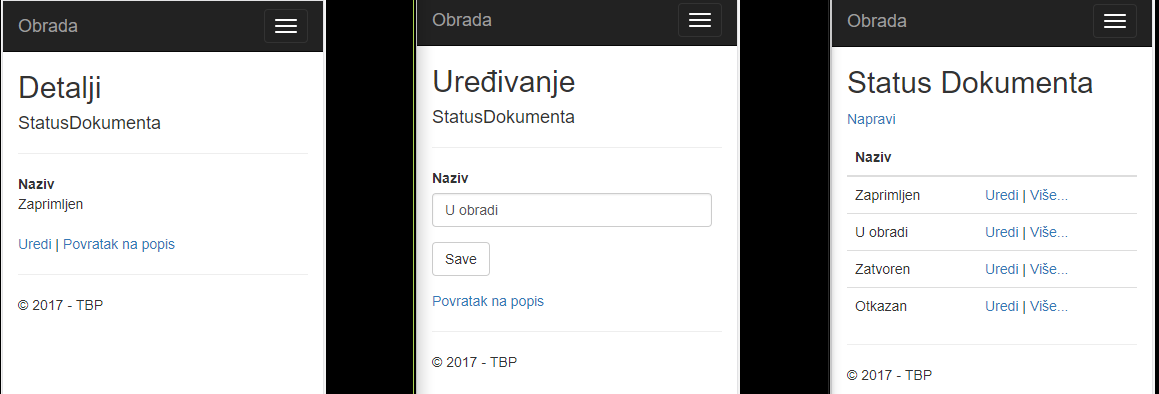
\includegraphics[width=0.95\textwidth]{sifrarnici.png}
\caption{Šifrarnici}
\label{slika-4}
\end{figure}

\section{Matični podaci}

Matični podaci su od ključnog značaja i trebali bi biti dostupni unutar cijelog sustava, a ne samo unutar djela za naručivanje, zaprimanje i izdavanje lijekova koji se ovdje obrađuje. Na slici 6.3 je prikazan padajući izbornik s matičnim podacima.


\begin{figure}[h]
\centering 
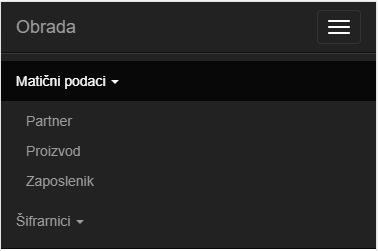
\includegraphics[width=0.5\textwidth]{maticni_podaci.png}
\caption{Matični podaci}
\label{slika-5}
\end{figure}

Matični podaci, kao što je vidljivo sa slike su Partner, Proizvod i Zaposlenik. Svi imaju specifična polja iz svoje domene te su isti navedeni u poglavlju o samom modelu. Sve se može uređivati, pregledavati popis i detalje, dok za partnera se može dodavati više kontakata što je nešto drugačije od ostalih pa su odabrani prikazi ekrana za rad s partnerima unutar matičnih podataka. Prvo se odabere kontakt s popisa i ode na uređivanje i nakon toga se odabere Dodaj kontakt gdje nam se otvara modalni prozor za unos kontakta, kao što je i prikazano na slici 6.4.

\begin{figure}[h]
\centering 
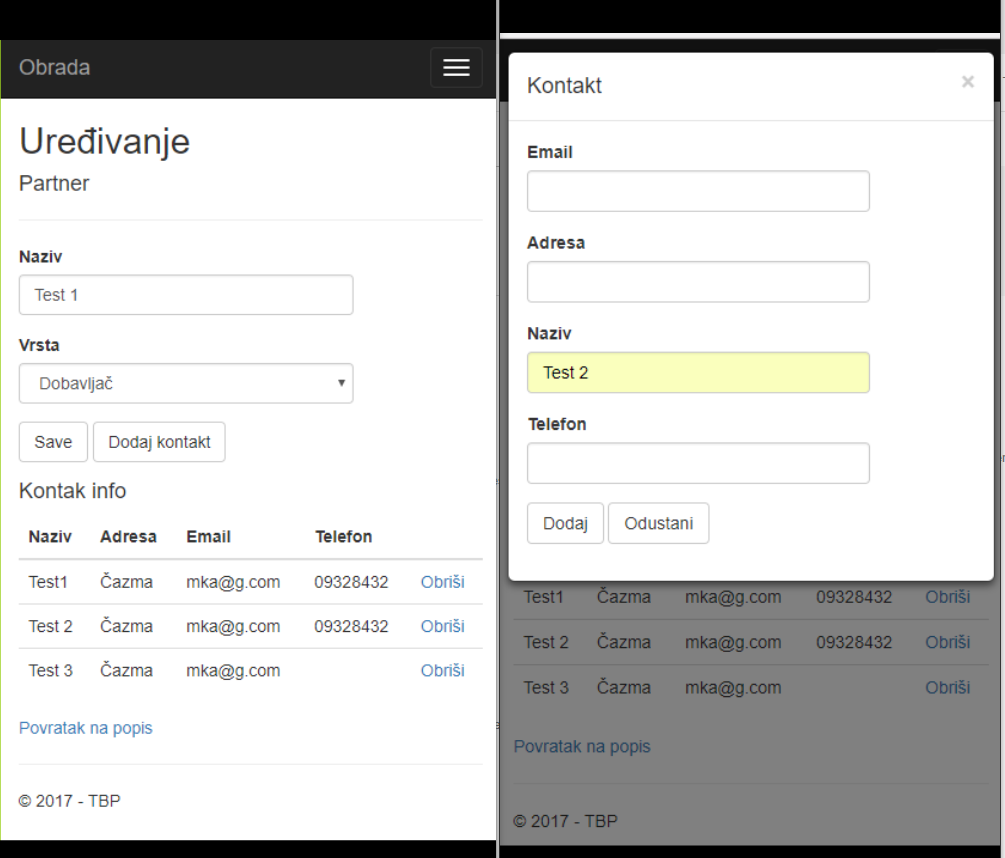
\includegraphics[height=0.55\textwidth]{uredivanje_partner_kontakt.png}
\caption{Uređivanje partnera}
\label{slika-6}
\end{figure}

\section{Obrada dokumenata}

Obrada dokumenta je sama esencija aplikacije. Sadrži se od nekoliko jednostavnih koraka. Osim, naravno samog pregleda i uređivanja, koji postoji za sve entitete te je zbog konzistentnosti ekran jednak kao i drugi, osim svojih specifičnosti. Korisnik ima gumb generiraj narudžbenicu koja generira sve stavke do maksimalnih količina te nas vodi na pregled same generirane narudžbenice i ukoliko želimo možemo je i uređivati. Možemo maknuti stavke ili promijeniti količine i sl. Nakon što smo gotovi s obradom narudžbenice mijenja se status u zatvoren. Nakon toga se može direktno iz narudžbenice generirati primka na temelju narudžbenice koju isto tako možemo urediti i sl. te ako smo sve zaprimili, ista se zatvara. Tu je sada završeno zaprimanje proizvoda (lijekova). Sada te iste lijekove izdajemo putem izdatnice za svaku ordinaciju ili direktno za pacijenta. I to je slijed aplikacije. Može se tu još puno stvari dodati, no ovo je konceptualne naravi i prikazano je s tehničke strane kako funkcionira. Sa samim generiranjem narudžbenice u biti možemo dobiti izvještaj što i koliko fali lijekova u bolnici.

\paragraph{Korak 1}
Na pregledu dokumenata se odabere akcija "Generiraj narudžbenicu".

\begin{figure}[h]
\centering 
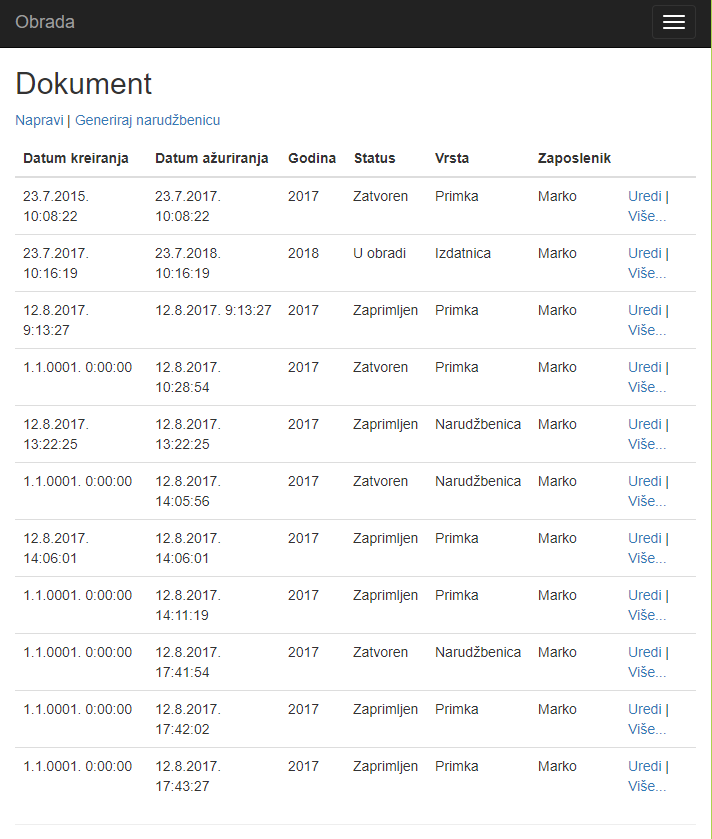
\includegraphics[height=0.95\textwidth]{dokument_pocetna.png}
\caption{Pregled dokumenata}
\label{slika-7}
\end{figure}

\paragraph{Korak 2}
U samoj narudžbenici se odabere akcija "Generiraj primku iz narudžbenice".

\begin{figure}[h]
\centering 
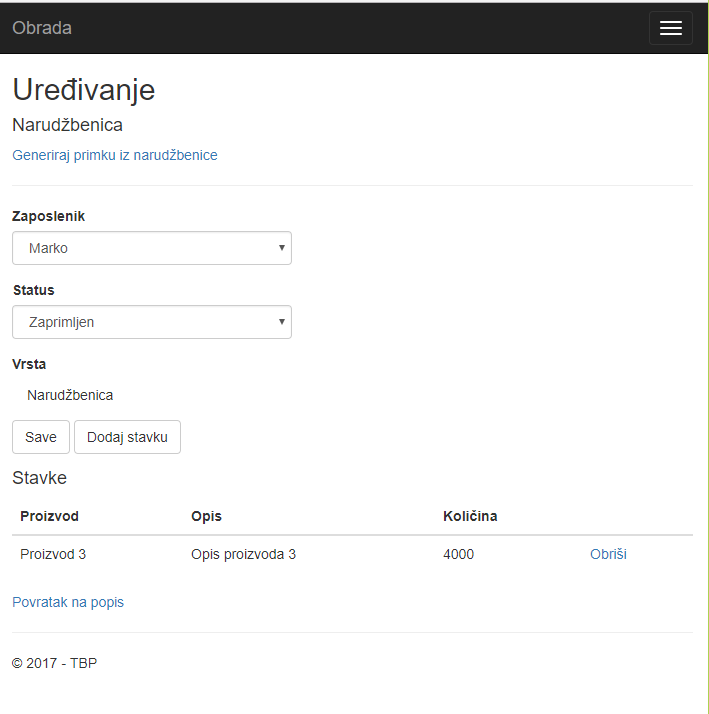
\includegraphics[height=0.50\textwidth]{dokument_narudzbenica.png}
\caption{Narudžbenica}
\label{slika-8}
\end{figure}

\paragraph{Korak 3}
Nakon zaprimanja i unosa točno zaprimljenih vrijednosti, primka se pohranjuje i zatvara.

\begin{figure}[h]
\centering 
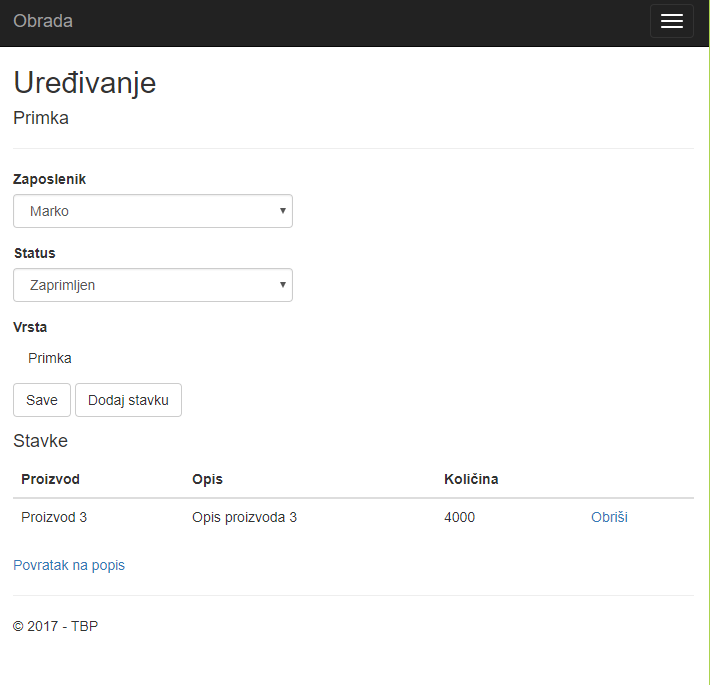
\includegraphics[height=0.50\textwidth]{dokument_primka.png}
\caption{Primka}
\label{slika-9}
\end{figure}

\chapter{Zaključak}

U današnje doba informatizacije želi se što više stvari automatizirati, no još važnije je prije što više unificirati jer će onda biti daleko lakše automatizirati. Kao sloj podataka koristila se baza podataka PostgreSQL koja je vrlo moćna i popularna u stvarnom svijetu. Ovdje su se koristile aktivne baze podataka, tj. okidači koji automatski odrađuju dio posla. Ja ne preferiram okidače, jer je vrlo teško za održavati, već većinu volim procesirati u aplikaciji. Naravno da za neke stvari ima smisla koristiti okidače, no treba biti vrlo oprezan s istima. Kao sloj prezentacijske i poslovne logike koristio se Microsoft .Net Core. Ova platforma je u dosta ranoj fazi, i kako se nisam još susreo u poslovnom svijetu s istom htio sam eksperimentirati i ovo mi je bila prilika. .Net Core se može izvršavati na svim operacijskim sustavima i serverima, što je velika novost za Microsoft kompaniju. Morali su se odlučiti za taj korak jer su uvidjeli da se tržište daleko jače razvija u svijetu otvorenog koda. .Net Core ima međusloj zvan Kestrel koji komunicira sa serverom, tako da je ovo mjesto gdje se spaja s OS-om i serverom. Osim navedenog, postoji još jedna velika prednost, a to je korištenje Entity Framework ORM platforme. EF je moćan i optimiziran ORM, te ga je jako jednostavno koristiti. Dakle, ovo ovdje napravljeno je bilo nespojivo do prije 2 godine: .Net MVC, PostgreSQL, EntityFramework, Linux. Ovaj rad nije rad koji može poslužiti u praksi, već više kao istraživački rad ("Proof of concept").


\addcontentsline{toc}{chapter}{Bibliografija}
\bibliography{foi}
\end{document}
